\chapter{Emergent inequality in a simple behavioral macroeconomic model}
\label{chapter:savings}

In this chapter I analyze the role of agent heterogeneity in a simple economic investment model where agents use a social learning heuristic to set their individual savings rates. To this end, I use a simplification of the heterogeneous agent investment model introduced in the previous chapter. This model is equivalent to an extension of the standard Ramsey-Cass-Koopmans (RCK) model to heterogeneous bounded rational households. Unexpectedly, this extended model is capable of producing endogenous oscillations in economic output resembling a business cycle. This is noteworthy as standard economic models usually depict business cycles not as endogenous dynamics but as the result of repeated exogenous shocks. In section \ref{sec:savings_introduction}, I motivate the use of heterogeneous bounded rational agents in economic growth and savings models to study emergent endogenous dynamics. Subsequently, I discuss the standard RCK model in section \ref{sec:savings_standard_rck} which is one of the foundational economic growth models. Based on this model, I give the specifications of the simplified agent-based heterogeneous household savings model in section \ref{sec:savings_model}. I present results of numerical simulations of the adapted model in section \ref{sec:savings_results} and discuss two different dynamical regimes of the model as well as the transition between them before concluding.

\section{Introduction}
\label{sec:savings_introduction}

Economic growth and inequality are important problems in economics \citep{Acemoglu2009, piketty2015capital}. Standard macroeconomic models are based on the assumption of a single representative rational utility maximizing agent and assume that the dynamics of business cycles are driven by exogenous shocks. However, empirical evidence from behavioral economics indicates that real households are heterogeneous and make substantial deviations from rationality.   This has led to new directions of research, including the incorporation of heterogeneous or bounded rational agents into macroeconomic models. This is typically done by allowing the agents to differ in terms of factors such as education while preserving the assumption of rationality \citep{ hank_reviewLeahy2018, hank_branch2009new, hank_zhao2018many}, or alternatively allowing for bounded rationality but maintaining utility maximization \citep{hank_gabaix2016behavioral}.  Realism is injected through imposing frictions, such as sticky wages.  These models require shocks to generate economic dynamics.

However, it has long been known that endogenous dynamics are possible in economic models~\citep{day1983emergence,BOLDRIN198626, Scheinkman, boldrin1992equilibrium, boldrin1992sources,blume1992evolution}, and more recently Beaudry \textit{et al.}\ have shown how limit cycles can emerge in a standard framework where agents are perfect utility maximizers \citep{beaudry2015reviving, beaudry2016putting}.  An alternative approach bases household decision making on simple heuristics rather than rationality \citep{DeGrauwe2011,DeGrauwe2010the}.  This leads to ``waves'' of optimism and pessimism, generating irregular business cycles and giving fat-tailed distributions for economic outcomes such as GDP. This chapter further develops this line of research by demonstrating how a very simple heterogeneous behavioral macroeconomic model leads to an endogenous business cycle that is not driven by externally imposed shocks. The purpose here is not to make a fully realistic model, but rather to demonstrate that rich emergent behavior can occur even under very simple assumptions.

This is done by extending the RCK model, which is one of the foundational models of economic growth theory. In this model a representative agent rationally chooses a savings rate in order to maximize discounted consumption.  However, there is ample evidence that households do not act as intertemporal optimizing agents and often respond myopically~\citep{Benartzi1995,Loewenstein2000,Choi2016}.  Evidence from lab experiments suggests that individuals perform poorly in finding optimal consumption paths. For instance, subjects deviated from optimal consumption choices by roughly 30 percent on average, increasing to roughly 50 percent when subjects were shown the average consumption level in the previous period  \citep{carbone2014lifecycle}.  Learning from past generations' consumption paths is somewhat more successful, but the errors are still substantial \citep{ballinger2003precautionary,brown2009learning}.  

Here, I take the opposite approach and assume a strong form of bounded rationality.  In this model households are embedded in a social network and make their savings decisions by simply copying their most successful neighbor. They do this episodically and myopically: From time to time they check all their neighbors and adopt the savings rate of the neighbor with the highest consumption.   

Although I do not claim that this behavior is fully realistic, there is empirical justification for considering a simple rule of this type.  The agents can be viewed as short-sighted, profligate ``conspicuous consumers'', and the tendency of households to copy one another has been well-documented since the time of Thorstein Veblen \citep{veblen1899}.  Imitate-the-best is one of the decision-making heuristics often applied in settings of high uncertainty and variability~\citep{Gigerenzer2011} and is observed in economic experiments~\citep{Traulsen2010}.  Savings behavior is highly dependent on social interaction with peers~\citep{Lu2011,Zhang2018,Kaustia2012, cascades} and comparing consumption levels incorporates the visibility bias and selection neglect observed in savings rate decisions~\citep{enke2015you}.  This implementation by copying based on consumption alone is partly motivated by the fact that a neighbor's consumption is more visible than their capital.    This makes it particularly surprising that in some circumstances their average behavior can be close to optimal.

I find that a key parameter governing economic behavior is the average time interval $\tau$ at which households update their savings rate, which I call the \textit{social interaction time}.  When $\tau$ is small, meaning the households update frequently, the savings rate is low, and the performance of the economy is suboptimal in terms of aggregate consumption. When $\tau$ is sufficiently large, in contrast, the economy-wide aggregate savings rate, which equals the income-weighted average household savings rate, becomes close to the optimal rate.  For small $\tau$ the population of households remains homogeneous, but as $\tau$ increases there is a sharp phase transition at a critical value $\tau_{c}$ where the population becomes strongly bimodal, dividing into rich households with high savings rates and poor households with low savings rates.  Correspondingly, for low values of $\tau$ the GDP and other economic indicators are constant with only small fluctuations, whereas above the critical transition there is an endogenous aperiodic oscillation, resembling a business cycle, in which the aggregate savings rate fluctuates, the population of households alternately becomes richer or poorer, and economic output varies substantially over time.  

This model shows that the use of heterogeneous agents following explicit behavioral rules can produce aggregate behavior that is qualitatively different from that of rational agents. This model is only qualitative, but its results suggest that an approach that explicitly incorporates empirical behavioral knowledge into household decision making may naturally lead to an explanation of business cycles in terms of endogenous dynamics. 
\newpage
\section{The Standard Ramsey-Cass-Koopmans model}
\label{sec:savings_standard_rck}

The following formulation of the standard Ramsey-Cass-Koopmans (RCK) model is based on refs. \cite[p. 287--317]{Acemoglu2009}, \cite[p. 85--135]{Barro2004}  and \cite[p. 38--90]{Blanchard1989} and uses continuous time, as in the original study \citep{Ramsey1928}.

Like many economic models, the standard RCK model studies the behavior of only one, infinitely lived, ``representative'' household with a strictly increasing and strictly concave utility function $u(c)$ depending only on consumption $c$. This household supplies labor $L$ and capital $K$ to a single representative firm that produces a single good $Y$ assuming a Cobb--Douglas production function
\begin{equation}
  Y \! =\! K^\alpha L^{1-\alpha}\label{eq:CD-Production}
\end{equation} 
with capital and labor elasticities $\alpha, 1 \!- \! \alpha \in (0,1)$.
In contrast to the original formulation of the model, I abstract from modeling labor growth as this is not relevant to the dynamics that I am interested in.
Per-capita production, $y \! =\! Y/L$, is thus a function of per-capita capital, $k \! =\! K/L$, only such that $y \! =\! k^\alpha$.

The RCK model assumes fully competitive factor markets. Consequently, as already discussed in section \ref{sec:model_description}, the two factors are compensated according to their marginal products, resulting in wages and capital rents as follows:
\begin{align}
  &w = \frac{\partial Y}{\partial L} = (1 - \alpha) y, \label{eq:wages}\\
  &r = \frac{\partial Y}{\partial K} = \alpha y /k. \label{eq:capital_rents}
\end{align}
This also means that the produced good is fully redistributed to the representative household leaving the representative firm with no profits.
The main model parameters of interest are the savings rate $s \le 1$ (which is allowed to be negative to reflect borrowing) 
and capital depreciation rate $\delta > 0$. These parameters govern aggregate and per-capita capital growth as follows, 
\begin{equation}
        \dot{K} = s(rK + wL) - \delta K,
        \quad \dot k = \bar{r}k + w - c,
\label{eq:kdot}
\end{equation}
where $\bar{r}=r-\delta$ is the real return rate and $c=(1-s)(rk+w)$ is per-capita consumption.
The household is assumed to maximize its discounted aggregate utility
\begin{equation}
        \int_0^{\infty} \! \mathrm{d}t \, e^{-\rho t} u(c(t)), 
        \label{eq:int1}
\end{equation}
by choosing an optimal path $s(t)$ for the savings rate, where $\rho>0$ is its discount rate.
To avoid that the representative household borrows money to shift its future consumption to the present and then continuously rolls over the existing debt into the future, one imposes a so called `No-Ponzi-Game' (NPG) condition \citep[p. 292]{Acemoglu2009}:
\begin{equation}
  \lim_{t \rightarrow \infty} k(t) e^{-\int_{0}^{t}d\tau \bar{r}(\tau)} \geq 0
  \label{eq:NPG}
\end{equation}
This equation ensures that households do not borrow more than they eventually receive and is equivalent to the future capital having a positive present value.
Thus, the task of the household is to find a path $(k(t),c(t))$ that optimizes equation \eqref{eq:int1} and satisfies equations \eqref{eq:kdot}  and \eqref{eq:NPG}.

\subsection{The RCK model's steady state}

For the instantaneous utility, one assumes a constant relative risk aversion (CRRA) function parameterized by
\begin{equation}
  u(c) = (c^{1-\theta} -1)/(1-\theta)~\mathrm{where}~\theta \geq0~\mathrm{and}~ \theta \neq 1.
  \label{eq:carra}
\end{equation}
Solving the intertemporal optimization problem posed by eq.~\eqref{eq:int1} subject to the constraints given by eqs.~\eqref{eq:kdot} and \eqref{eq:NPG} with the utility function \eqref{eq:carra} results in the Ramsey-Keynes equation
\begin{equation}
  \frac{\dot{c}}{c} = \frac{\bar{r} - \rho}{\theta}
  \label{eq:ramsey_keynes}
\end{equation}
that gives the relative growth rate of consumption depending on the real return rate on capital $\bar{r}$, the households discounting rate $\rho$ and the elasticity of its marginal utility $\theta$.\\

In particular, this system has two steady states with $\dot c\!=\!0$, a trivial one in which $c\!=\!k\!=\!0$ and another in which 
the real return rate equals the discount rate, $\bar r \!=\! \rho$, corresponding to a modified `golden rule' \citep[p. 300]{Acemoglu2009}. In this non-trivial steady state capital, consumption and savings rate are given by
\begin{equation}
	k^\ast = \left(\frac{\alpha}{\rho + \delta}\right)^{\frac{1}{1-\alpha}}, 
 	\quad c^\ast = {k^\ast}^{\alpha} -  \delta k^\ast,
 	\quad s^\ast_\mathrm{RCK} = \frac{\alpha \delta}{\rho + \delta}. \label{eq:rck_steady_state}
\end{equation}
For the limit case $\rho\to 0$, this reproduces the Solow model's golden rule \citep[p. 35]{Barro2004}, 
\begin{equation}
  s^\ast_\mathrm{RCK} \! =s_\mathrm{gold} \!=\! \alpha.
  \label{eq:golden_rule}
\end{equation}
This is called the golden rule because $s = \alpha$ leads to the largest possible sustainable consumption,
\begin{equation}
        c^\ast \! =\!(1\! -\! \alpha)(\alpha/\delta)^{\alpha/(1-\alpha)}.
        \label{eq:golden_rule_consumption}
\end{equation}
For $\rho \! > \!0$, the discount rate pushes the households to save less and shift consumption towards the present, resulting in a smaller (and thus ex-post suboptimal) $c^\ast$ than in the Solow model.

Given the current value of per-capita capital $k$, the household chooses a current value of per-capita consumption $c(s)$ determined by intertemporal optimization, leading to an optimal consumption path that maximizes the household's long-term discounted aggregate utility.  This determines the time evolution of $k$ and $c$ 
towards a steady state at $(k^\ast, c^\ast)$.  


\begin{figure}[t]
  \begin{minipage}[c]{0.4\textwidth}

    \caption[]{From \cite[p. 100]{Barro2004}. Phase space of equations \eqref{eq:kdot} and \eqref{eq:ramsey_keynes} that is often times falsely discussed as the phase space of the RCK model. However, eq. \eqref{eq:NPG} confines the support of the solution of the RCK model to the saddle point manifold. Outside this saddle point manifold, eq. \eqref{eq:ramsey_keynes} does not hold.\label{fig:rck_phase_space}}
  \end{minipage}
  \begin{minipage}[c]{0.6\textwidth}
        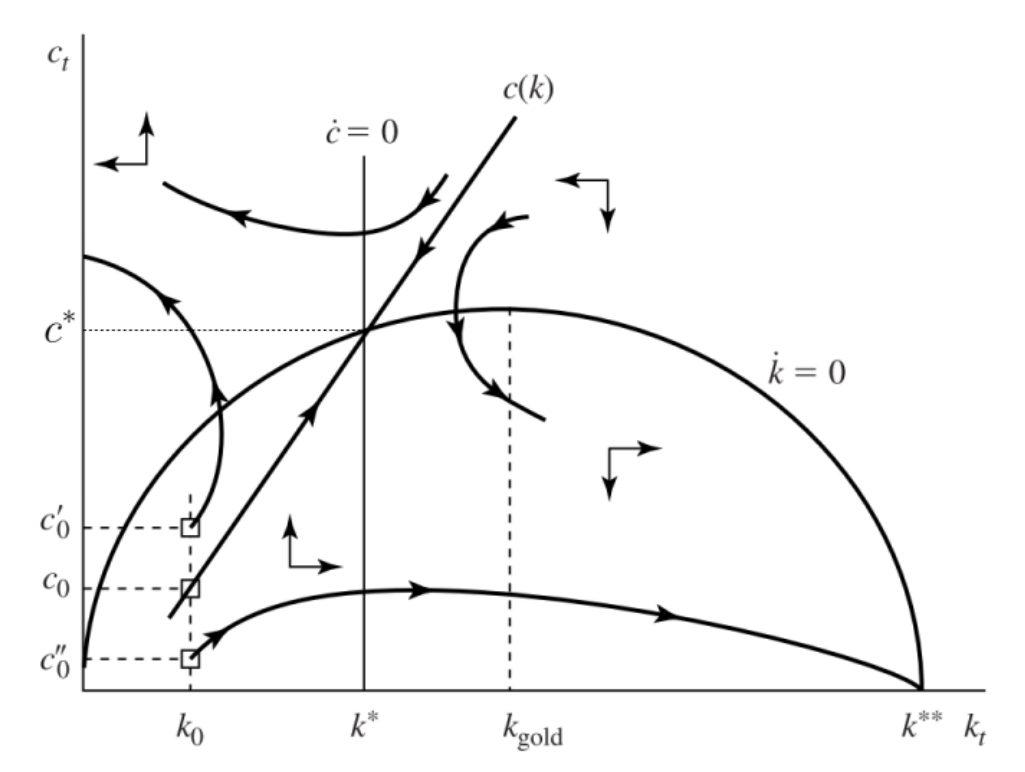
\includegraphics[width = 1 \textwidth]{./figures/RCK_phase_space.png}
  \end{minipage}\hfill

\end{figure}

From a physicist's perspective, eqs. \eqref{eq:kdot} and \eqref{eq:ramsey_keynes} resemble a system of ordinary differential equations that describe the dynamics of the RCK model in the $(k,~c)$ phase space. This line of reasoning would yield a phase space diagram like the one presented in fig.~\ref{fig:rck_phase_space} that exhibits trivial absorbing states along the axes $k=0$ and $c=0$ and two saddle points for $k=c=0$ and another one derived in eq. \eqref{eq:rck_steady_state}.
This view has some appeal as it allows for the framing of bubbles and crashes as deviations from the optimality curve and subsequent corrections to get back to it --- so much so that even economic textbooks feature figures like fig. \ref{fig:rck_phase_space} that clearly buy into this framing.
However, a closer look at the derivation of equation \eqref{eq:ramsey_keynes} reveals that this framing --- as attractive and intuitive as it seems --- is the product of circular reasoning and a flawed understanding of the mathematical optimization methods that are used to derive it. Particularly, the derivation of eq.~\eqref{eq:ramsey_keynes} is done by solving the intertemporal optimization problem posed by eq.~\eqref{eq:int1} subject to eq.~\eqref{eq:kdot} with eq.~\eqref{eq:NPG} with strict equality as a constraint. This constraint confines the solution of the optimization problem to the saddle point manifold in fig.~\ref{fig:rck_phase_space} which in return means that any discussion of this solution outside the saddle point manifold is meaningless. Consequently, any interpretation of the possible dynamics of equations \eqref{eq:kdot} and \eqref{eq:ramsey_keynes} that revolve around stability of the steady state, deviations from the manyfold and possible ways to return to it are meaningless as they are outside the support for which the ordinary differential equations were derived in the first place.

To sum up, this means that while the RCK model has been used extensively to study the effect of different policy measures on economic growth, its use for the study of non-equilibrium economic dynamics is somewhat limited. \\

An interesting extension of this model including heterogeneous agents and relaxing the rationality assumptions for their behavior can address this point. Subsequently, I introduce such a model.




\section{An Agent-Based Version of the RCK Model}
\label{sec:savings_model}
\subsection{Economic Model}
The model introduced in this chapter originated as a derivative and modification of the model described in section \ref{sec:heuristics_model}. The aim of this model is to answer some of the questions that I raised at the end of the previous chapter; namely, what effects may araise from heterogeneous agents individually setting their savings rates according to a simple social learning rule. In the following, I will explain the model in detail.\\

I introduce a heterogeneous agent model in the tradition of agent-based modeling \citep{LeBaron1999,Berry2002,Epstein2006,Dosi2010, Dawid2014,Hommes2018,Simon2018},
using agents that follow a very simple behavioral rule.  
This model contains $N$ households labeled by $i$ with heterogenous capital $K_i$. For simplicity, all households supply the same labor $L_i = L/N$.  \footnote{Introducing heterogeneous labor has little effect on the results}.
As in the original RCK model, total economic production is given by the Cobb--Douglas production function, in this case applied to the aggregate input factors $K = \sum_{i=1}^N K_i$ and $L = N L_i$.
As in the original model, capital returns $r$ and wages $w$ equal marginal returns according to eq.~\eqref{eq:capital_rents},
but incomes $I_i$ now differ between households,
\begin{equation}
\label{eq:Ii}
	I_i = r K_i + w L/N.
\end{equation}

The key assumption is that each household individually and dynamically sets its time-dependent savings rate $s_i(t)$ according to a behavioral decision rule introduced below,
leading to household capital dynamics
\begin{equation}
	\dot{K}_i = s_i I_i - \delta K_i = (r s_i - \delta) K_i + w s_i L/N.
        \label{eq:rcka_kdot}
\end{equation}
At the steady state where $\dot{K}_i = 0$, the steady state value $K_i^*$ for household $i$'s capital is a function of the aggregate capital $K$ via its dependence on $w$ and $r$, 
nonlinearly interconnecting all the agents' savings rates and consumption levels.

\subsection{Household Decision Making}
While the standard RCK model is a one-dimensional dynamical system in which consumption is a deterministic function of the total capital, the agent-based version is $N$-dimensional, and aggregate consumption depends on all households.
I assume that each household updates its savings rate at random times\footnote{
%
This leads to smoother transitions than synchronous updates \citep{Vizzari2005, Fates2010}.
}
%
according to a Poisson process with rate $1/\tau$.

Households are embedded in a social network in which each household $i$ has neighbors $\mathcal{N}(i)$. Inspired by a recent study on heuristic behavior in social learning by \cite{Barkoczi2016}, I implement household behavior in the following way: Whenever household $i$ updates its savings rate, it compares the consumption rates of its neighbors and applies the `imitate-the-best' heuristic, copying the savings rate of the neighbor with the highest current consumption with a small deviation that can either be interpreted as an error or as an exploration \citep{Mehlhorn2015}. More precisely, when the consumption of a neighbor is higher, it adopts a new savings rate of
\begin{equation} 
	s^\mathrm{new}_i = s_{\underset{j\in \mathcal{N}(i)}\argmax_{} (C_j)} + \epsilon,
\end{equation}
where $\epsilon$ is distributed uniformly in the interval of $\pm 1\%$\footnote{With $\varepsilon=0$ the values of the savings rate the households can use are confined to the values that occur in the initial condition. Also, values of the savings rate can ``die out'' as soon as the last household has abandoned them. This leads to strong and artificial path dependencies. The model behavior is insensitive to to exact value of $\varepsilon$ as long as there is some diversity e.g. $\varepsilon>0$}.
Note that in this model household savings rates are strictly non-negative. While this excludes effects that may come from borrowing between households, it  also serves as a simple and robust alternative for the No-Ponzi-Game condition that lies at the heart of the original RCK model. 

\subsection{Simulation Details}

For the simulations that are presented in the subsequent results section, the parameters and initial conditions are as follows if not explicitly stated otherwise:
$L_i = 1/N, K(t=0)_i \!= \!1 \forall\,\, i$ and a fully connected network with $N=100$, $\delta=0.05$. We have found that adding small heterogeneity in each household's labor does not change the dynamics significantly and the equilibrium dynamics also remain the same for different initial capital distributions with different $\sum_i K_i = K$. We used Gillespie's algorithm \citep{Gillespie1977} to simulate the stochastic trajectory.

\section{Results}
\label{sec:savings_results}
I present the results as follows: First I show the model dynamics depending on the mean social interaction time $\tau$ and classify them according to two qualitatively different regions. I consecutively analyze these two regions with respect to their dynamic properties and explain the underlying mechanisms. Finally, I explain the origin of the critical social interaction time that separates the different dynamical regimes and discuss its dependency on the structure of the interaction network.\\
\begin{figure}[ht]
     \centering
     \vspace{-.2 cm}
     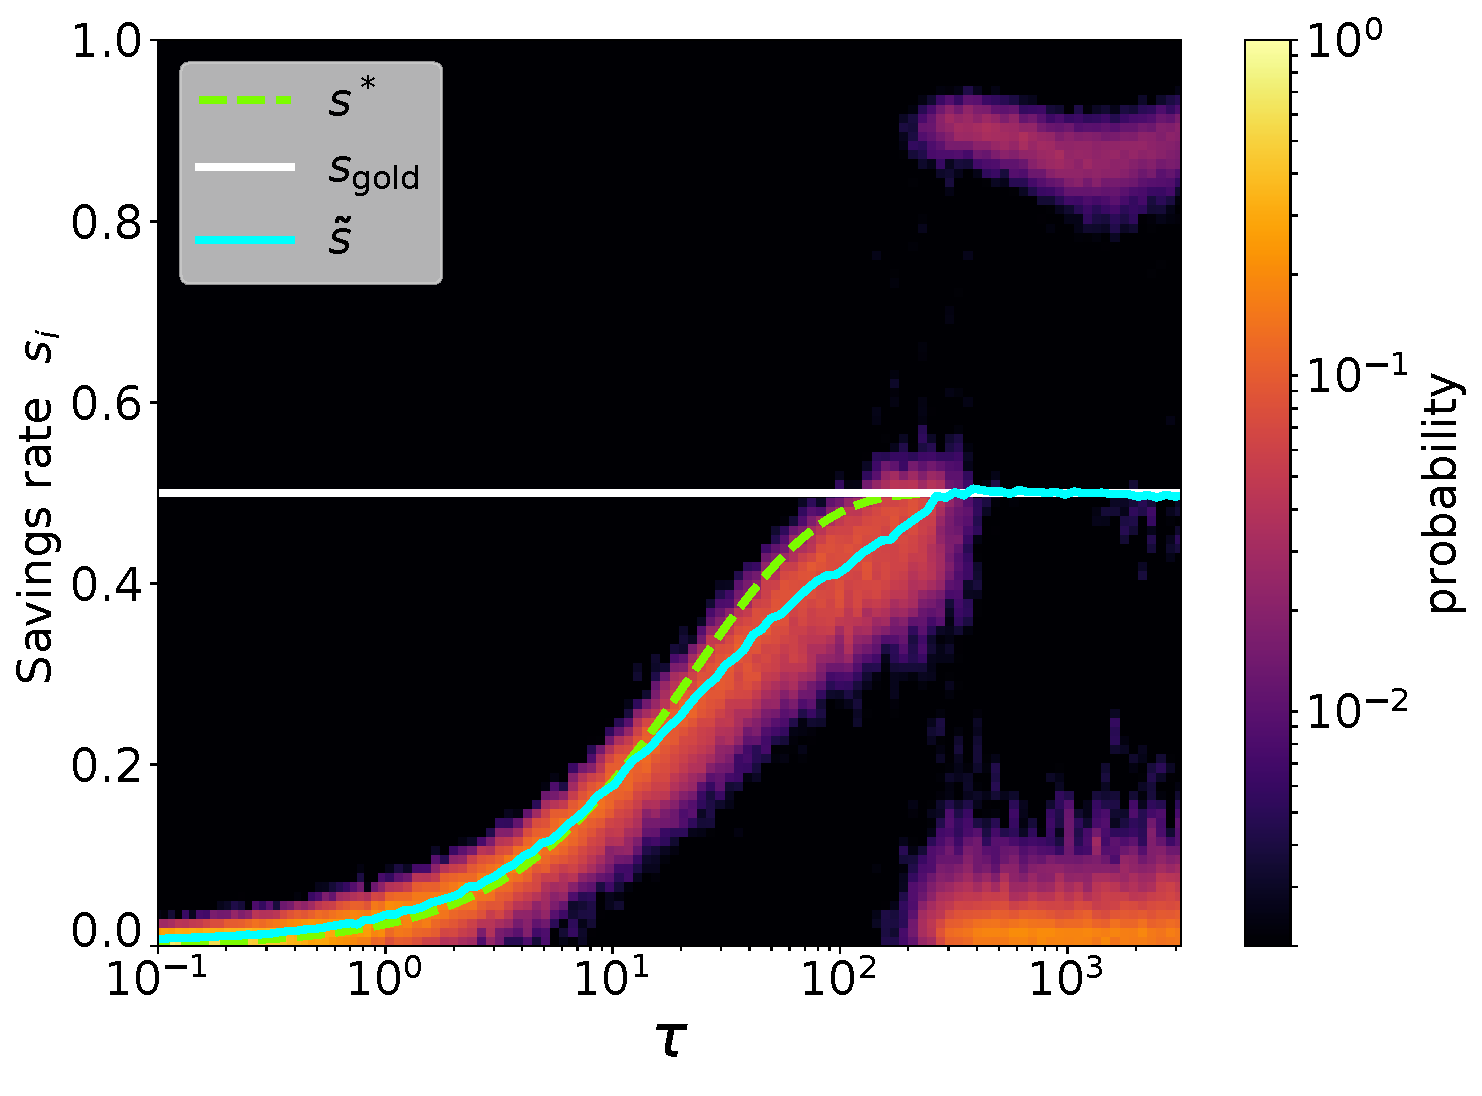
\includegraphics[width=.9\linewidth]{figures/fig1.pdf}
	\caption []{{ The critical transition from the stable regime to the oscillatory regime.} 
	 Results from an ensemble of simulations at different values of the social interaction time $\tau$, with other parameters held fixed. The savings rate distributions are shown at the final state of the simulation at time $5\tau \times 10^3$, far beyond the point where the model has reached its asymptotic dynamics. For each value of $\tau$, $200$ independent simulations are run and all values of $s_i$ are recorded for each $\tau$ to construct a normalized histogram.
       The heatmap indicates the probability density of the distribution of individual households savings rates for each value of $\tau$, along with the aggregate savings rate $\tilde{s}$. This is compared to the golden rule savings rate $s_\mathrm{gold} \! = 0.5$ and the savings rate $s^*$ predicted by eq.~(\ref{eq:s_optimal}).}
	
   \label{phase}
\end{figure}
We simulated the model for a variety of different parameters such as the average social interaction time $\tau$ and the network topology. Fig.\,\ref{phase} shows the distribution of the final savings rates as a function of the mean social interaction time $\tau$ for a complete network with the remaining parameters fixed.  The figure compares this result to the optimal, `golden rule' savings rate $s_\mathrm{gold}$,  corresponding to the rational expectations equilibrium where the consumption of the representative agent is maximized. For comparison, the figure also shows the analytical approximation of the steady state savings rate of the model $s^*$ in eq. \eqref{eq:s_optimal}.\\

These results clearly show that there are two distinct regimes, separated by a critical social interaction time $\tau_{c} \approx 250$.
In the \emph{stable regime}, corresponding to $\tau < \tau_{c}$, the savings rates of the households are unimodally distributed around a low savings rate.  For very small values of $\tau$ the savings rates are close to zero, and because of this, the economy is stuck in a poverty trap in which its output is very low.  As $\tau$ increases, the savings rate and output increase, but the distribution remains unimodal, with a sub-optimal aggregate savings rate.

For $\tau \! > \! \tau_{c}$ the economy enters what I call the \emph{ oscillatory regime}, where the behavior is dramatically different. In this regime the savings rate distribution is bimodal --- some households have high savings rates and are :``wealthy'', while others have low savings rates and are ``poor''.  Thus, this model exhibits spontaneous emergence of extreme inequality, with a lower class and an upper class.

Very near $\tau_\mathrm{c}$ the distribution in fig.~\ref{phase} becomes tri-modal. This is due to intermittent oscillations between the unimodal and bi-modal regimes. Thus the system either exhibits a middle class, or a lower class and an upper class, but never all three at once.

Strikingly, as long as $\tau \! > \! \tau_{c}$, the ensemble average of the observed economy wide aggregate savings rate $\tilde{s}$ is within $1\%$ of the optimal value $s_\mathrm{gold}=\alpha=0.5$, even when the individual distributions are bimodal.
Furthermore, the time averages of total economic output $Y(t) \!=\! 10.15$ and  consumption $C \! = \! 4.99$ are close to their optimal values $Y^\ast \! = \! s_\mathrm{gold} L/\delta \! = \! 10$  and $C^\ast \! = \! (1-s_\mathrm{gold})Y^\ast \! = \! 5$  in the standard RCK model.  It is surprising that such a simple, near zero-intelligence learning rule can maintain the system this close to its optimal behavior.
\begin{figure}[t]
     \centering
       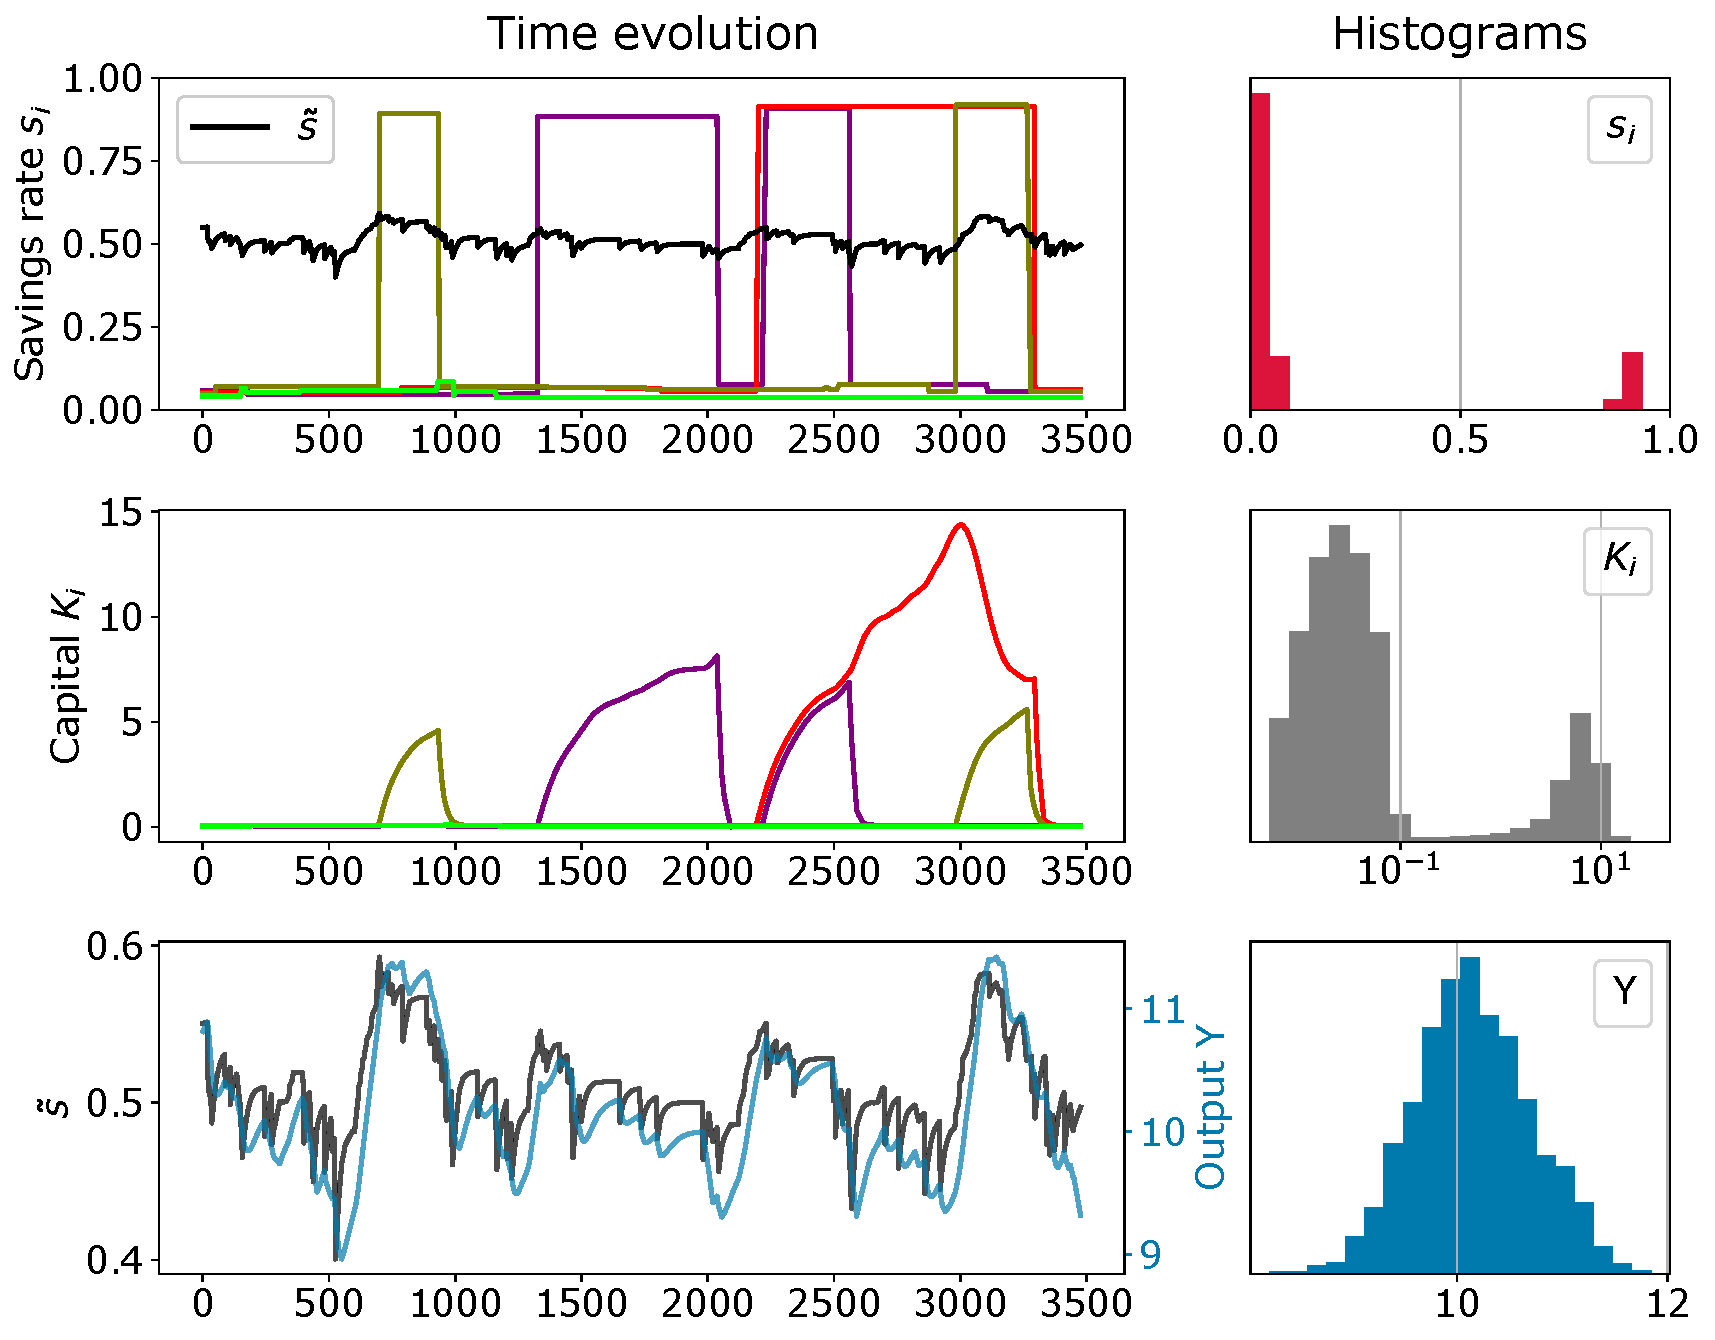
\includegraphics[width=0.99\linewidth]
       {figures/fig2.pdf}
	\caption{{ The endogenous business cycle in the oscillatory regime}.   I show several time series for $\tau \!>\! \tau_\mathrm{c}$.  
	The top left panel shows the savings rates $s_i(t)$ for randomly chosen households as a function of time, as well as the aggregate savings rate $\tilde{s}$.  
	The middle left panel shows the capital $K_i(t)$ of the same households as a function of time. The bottom left panel shows the cyclic behavior of the aggregate output superimposed on the aggregate savings rate.  The panels on the right are histograms of the indicated variables, accumulated over a longer interval.}
   \label{fig:micro_trajs}
\end{figure}

The system dynamics become clearer when analyzing the properties of the 
economy as a function of time, as illustrated in fig.~\ref{fig:micro_trajs}.  
For $\tau \! > \! \tau_\mathrm{c}$ there is an endogenous oscillation in many of the aggregate properties of the economy, including the aggregate savings rate $\tilde{s}(t)$ and output $Y(t)$.  This oscillation is also visible in the behavior of individual households.  If one follows any single household it experiences epochs with both, a high savings rate near $s_i \! \approx \! 0.90$, and a low savings rate near $s_i \! \approx \! 0.05$.  At any point in time there is typically an imbalance between rich households and poor households, so that the aggregate savings rate and the aggregate output fluctuate.  I loosely refer to this endogenous oscillation as a ``business cycle''.
%In the Supplementary Information (SI) we show that the value of the high savings rate varies between $65\%$--$90\%$ depending on the topology of the network.  


\subsection{Understanding the Stable Regime ($\mathbf{\tau \! < \! \tau_{c} }$)}
\label{sec:savings_stable}
Although the behavioral rule of the `imitate-the-best' heuristic requires minimal intelligence, the selection process of copying the household with the highest consumption provides a simple mechanism of collective search that becomes more effective as the social updating time $\tau$ increases.  This is perhaps counter-intuitive, as it means that inattention results in superior collective outcomes. The underlying explanation is as follows:  The  savings rate of the household that is copied has on average been fixed for a time interval of order $\tau$. When $\tau$ is small, planning is too myopic, ``short term thinking'' dominates, and the households cannot escape using low savings rates with high consumption.  As $\tau$ increases, however, the time between updates becomes long enough that there is more time to accrue an advantage by saving. This drives the savings rate up and increases economic output. The competitive selection process guarantees that for a sufficiently large population and large $\tau$ the savings rates are close to optimal. This is similar to the behavior of a model of local resource exploitation \citep{Wiedermann2015}.

We can use this intuition to derive an approximate formula for the aggregate savings rate $s^*$ as a function of~$\tau$. This derivation takes advantage of the fact that in the stable regime the distribution is unimodal and assumes that all households have essentially the same savings rate. With this, one can derive the optimal savings rate for time horizon $\tau$ as follows.\\ 

\subsubsection{Analytical Approximation of the Stable Regime's Steady State}
\label{sec:rck_stable}
The main idea is the following: First, study which member of an ensemble of households  will have the largest consumption after the short time interval $\tau$ given that they all start at similar but slightly different savings rates. Then, assume all households will copy the savings rate of this best household with some error. 
This is only an approximation since in the actual model, households do not simultaneously imitate each other after an exact time $\tau$. Furthermore, the approximation will only be satisfactory when households have already converged to similar savings rates and capital stocks.
Nevertheless, the approximation describes the joint motion towards a steady state  rather well once households have converged towards each other.

To see how individual households' consumption at time $\tau$ depends on their individual savings rate, one has to approximate the evolution of $r$ and thus of total capital $K$ first. Let us assume that all households' savings rates $s_i$ are close to the overall savings rate $s$ and stay constant between time zero and time $\tau$. 
Then according to eq. \eqref{eq:rcka_kdot} $K$ evolves as 
\begin{equation}
    \begin{split}
    \dot K &= (r s - \delta) K + w s L \nonumber \\
    	   &= \Big(\alpha\Big(\frac{L}{K}\Big)^{1-\alpha} s - \delta\Big) K + \alpha \Big(\frac{K}{L}\Big)^{1-\alpha} s L.  
	\end{split}
\end{equation}
For $\alpha = 1/2$ this simplifies to 
\begin{equation}
    \label{aggKdotnew}
    \dot{K} = s\sqrt{L K} - \delta K.
\end{equation}
Assuming that $s$ does not change before time $\tau$, this can be solved via separation of variables which results in two solutions given by 
\begin{equation}
\begin{split}
    K(t) &= \Big(\frac{B - E e^{-\delta t/2}}{\delta} \Big)^2, \\
    r(t) &= \sqrt{L/K} / 2 = \frac{A}{B - E e^{-\delta t/2}}, \\
    w(t) &= \sqrt{K/L} / 2 = \frac{B - E e^{-\delta t/2}}{4 A}
\end{split}
\end{equation}
for all $t < \tau$,
where 
$A = \delta \sqrt{L} / 2$,
$B = s\sqrt{L}$,
and
$E$ has the two possible values $s\sqrt{L} \pm \delta \sqrt{K_0}$.
Since the only relevant solution is that in which $r$ is positive, we find $E = s\sqrt{L} - \delta \sqrt{K_0} < B$.

Knowing $r(t)$ and $w(t)$, we can now determine which household consumes most after time $\tau$.
Household $i$'s capital $K_i(t)$ evolves as 
\begin{equation}
\begin{split}
    \dot K_i 
    &= (s_i r(t) - \delta) K_i + w s_i L_i \nonumber \\
    &= \left(\frac{A}{B - E e^{-\delta t/2}} - \delta\right)s_i K_i
        + \frac{B - E e^{-\delta t/2}}{4 A} s_i L_i.
\end{split}
\end{equation}
This has an analytical solution involving complicated hypergeometric functions.
For small values of $\tau$, we can simplify the problem by approximating $r(t)$ and $w(t)$ for $t\in[0,\tau]$ by their mid-term values $r(\tau/2)$ and $w(\tau/2)$, giving
\begin{equation*}
\dot{K_i} \approx G_i K_i + F_i
\end{equation*}
with $G_i = \frac{s_i A}{B - E e^{-\delta \tau/4}} - \delta$
and $F_i = \frac{B - E e^{-\delta \tau/4}}{4 A} s_i L_i$,
which solves as
\begin{equation*}
    K_i(t) \approx (K_i(0) + F_i/G_i)e^{G_i t} - F_i/G_i.
\end{equation*}
The corresponding consumption of household $i$ at time $\tau$ is then
\begin{align}
    C_i(\tau) 
    &= (1 - s_i)(r(\tau) K_i(\tau) + w(\tau) L_i) \nonumber \\
    &\approx (1 - s_i)\left( 
        H((K_i(0) + F_i/G_i)e^{G_i\tau} - F_i/G_i)
        + L_i/4 H
    \right)
\label{eq:Citau}
\end{align}
with 
\begin{equation}
        H = \frac{A}{B - E e^{-\delta\tau/2}} = \frac{A}{s\sqrt L (1 - e^{-\delta\tau/2}) + \delta \sqrt{K_0} e^{-\delta\tau/2}}.\nonumber
\end{equation}
%Note that $F_i/G_i$ decreases as $s_i$ increases.
We assumed that at time $\tau$ all households imitate the savings rate $s_i$ that has led to the largest $C_i(\tau)$. This means that as long as a single household can increase its consumption $C_i(\tau)$ by choosing a savings rate $s_i$ that is similar to but different from $s$, all households will imitate this savings (with some error) rate and the aggregate savings rate will move towards $s_i$. 
We can also determine whether $s$ will increase or decrease by identifying whether the $s_i$ that gets copied is larger or smaller than $s$.
Since we also assume households' savings rates $s_i$ are distributed closely around $s$, and that all $K_i(0), L_i$ are similar, this can be determined by seeing whether $C_i(\tau)$ increases or decreases when $s_i$ is increased from below $s$ to above $s$, i.e., by studying the derivative $\partial C_i(\tau)/\partial s_i$ at the point $s_i = s$. Up to a factor of $N$, this derivative is given by
\begin{align}
  \frac{\partial C_i(\tau)}{\partial s_i} = &(1 - s) H\left[
        \frac{e^{G\tau} - 1}{G}(L / 4 H - H F/G) + e^{G\tau}\tau H (K_0 + F/G)\right] \nonumber \\
    &- H[(e^{G\tau} - 1) F/G + e^{G\tau} K_0] 
    - L / 4 H
    \label{sdotnew}
\end{align}
where
$F = \frac{B - E e^{-\delta \tau/4}}{4 A} s L$
and
$G = \frac{s A}{B - E e^{-\delta \tau/4}} - \delta$.
As long as the above expression is positive or negative, $s$ will increase or decrease over time, respectively.

A steady state will then be reached when both $s$ and $K$ change no longer, i.e., when both $\dot K$ as given by eq.~\eqref{aggKdotnew} (with $K=K_0$) as well as $\partial C_i(\tau)/\partial s_i$ as given by eq.~\eqref{sdotnew}
vanish.
The solution of $\dot K = 0$ is 
$K_0 = L s^2 / \delta^2$, 
at which point we have
$E = 0$,
$H = \delta / 2 s$, 
$G = - \delta / 2$, 
$F/G = - L s^2 / \delta^2 = - K_0$, 
$H K_0 = L s / 2 \delta$, and
$H F / G = - L s / 2 \delta = - H K_0$.
Substituting all this into eq.\,\eqref{sdotnew} and equating it with zero gives the following surprisingly equation for the steady state $s$:

\begin{equation}
\label{eq:s_optimal}
s^\ast(\tau) = \frac{1 - e^{-\delta \tau/2}}{2 - e^{-\delta \tau/2}}.
\end{equation}
This approximation describes the aggregate macroscopic behavior of the model in the stable regime. It illustrates that this macroscopic behavior is determined by the relative time scales of the two major processes in this model, the capital depreciation rate $\delta$ in the economic system that determines the transient dynamics of capital accumulation through savings and the social interaction time $\tau$ that determines the speed of collective search in the social learning process. Such behavior is common for many coupled dynamical systems. [Maybe some citations here.] This approximation is shown in green in fig.~\ref{phase} comparing it to the aggregate savings rate and the distribution of individual savings rates from numerical simulations. This shows that this analytical approximation provides a good fit of the aggregate savings rate throughout the stable regime.

The analytical approximation of the aggregate savings rate in the stable regime of the agent-based RCK model can be compared to the optimal savings rate in the steady state of the standard RCK model. In the standard RCK model as given in eq.~\eqref{eq:rck_steady_state}, the optimal savings rate depends on the capital depreciation rate $\delta$ and the discount rate $\rho$, which is a free parameter. Substituting $s^\ast$ from eq.~\eqref{eq:s_optimal} into the relation for the classical RCK model from eq. \eqref{eq:rck_steady_state} and solving for $\rho$ gives an effective discounting rate for this model in terms of the social interaction time $\tau$ and the depreciation rate $\delta$,
\begin{equation}
   \rho(\tau) = \frac{\delta/2}{e^{\delta \tau/2} - 1}. \label{eq:rhotau}
\end{equation}
In the limit of $\tau \to 0$, the discount rate $\rho$ diverges, consistent with the observed collectively myopic behavior. But for $\tau \to \infty$, the discount rate $\rho$ converges to zero consistent with collectively farsighted behavior and an optimal savings rate in the sense that this would be the savings rate that a social planner would choose to achieve the highest sustainable aggregate consumption. Thus in this case the individually myopic households act collectively ``as if'' they were farsighted, with an emergent effective discounting rate $\rho(\tau)$ which is not a free parameter but is rather a function of the social interaction time $\tau$. Similar emergent behavior has been found in the interaction of adaptive voter type social learning with individual management of renewable resources where sustainable far sighted management of the resource is possible when the interaction time in the social learning process is sufficiently large compared to the time scale of the inherent dynamic renewable resource \citep{Wiedermann2015}. 


\subsection{Understanding the oscillatory regime ($\mathbf{\tau \!>\! \tau_{c} }$)}
\label{sec:savings_oscillations}


\begin{figure}[t]
     \centering
       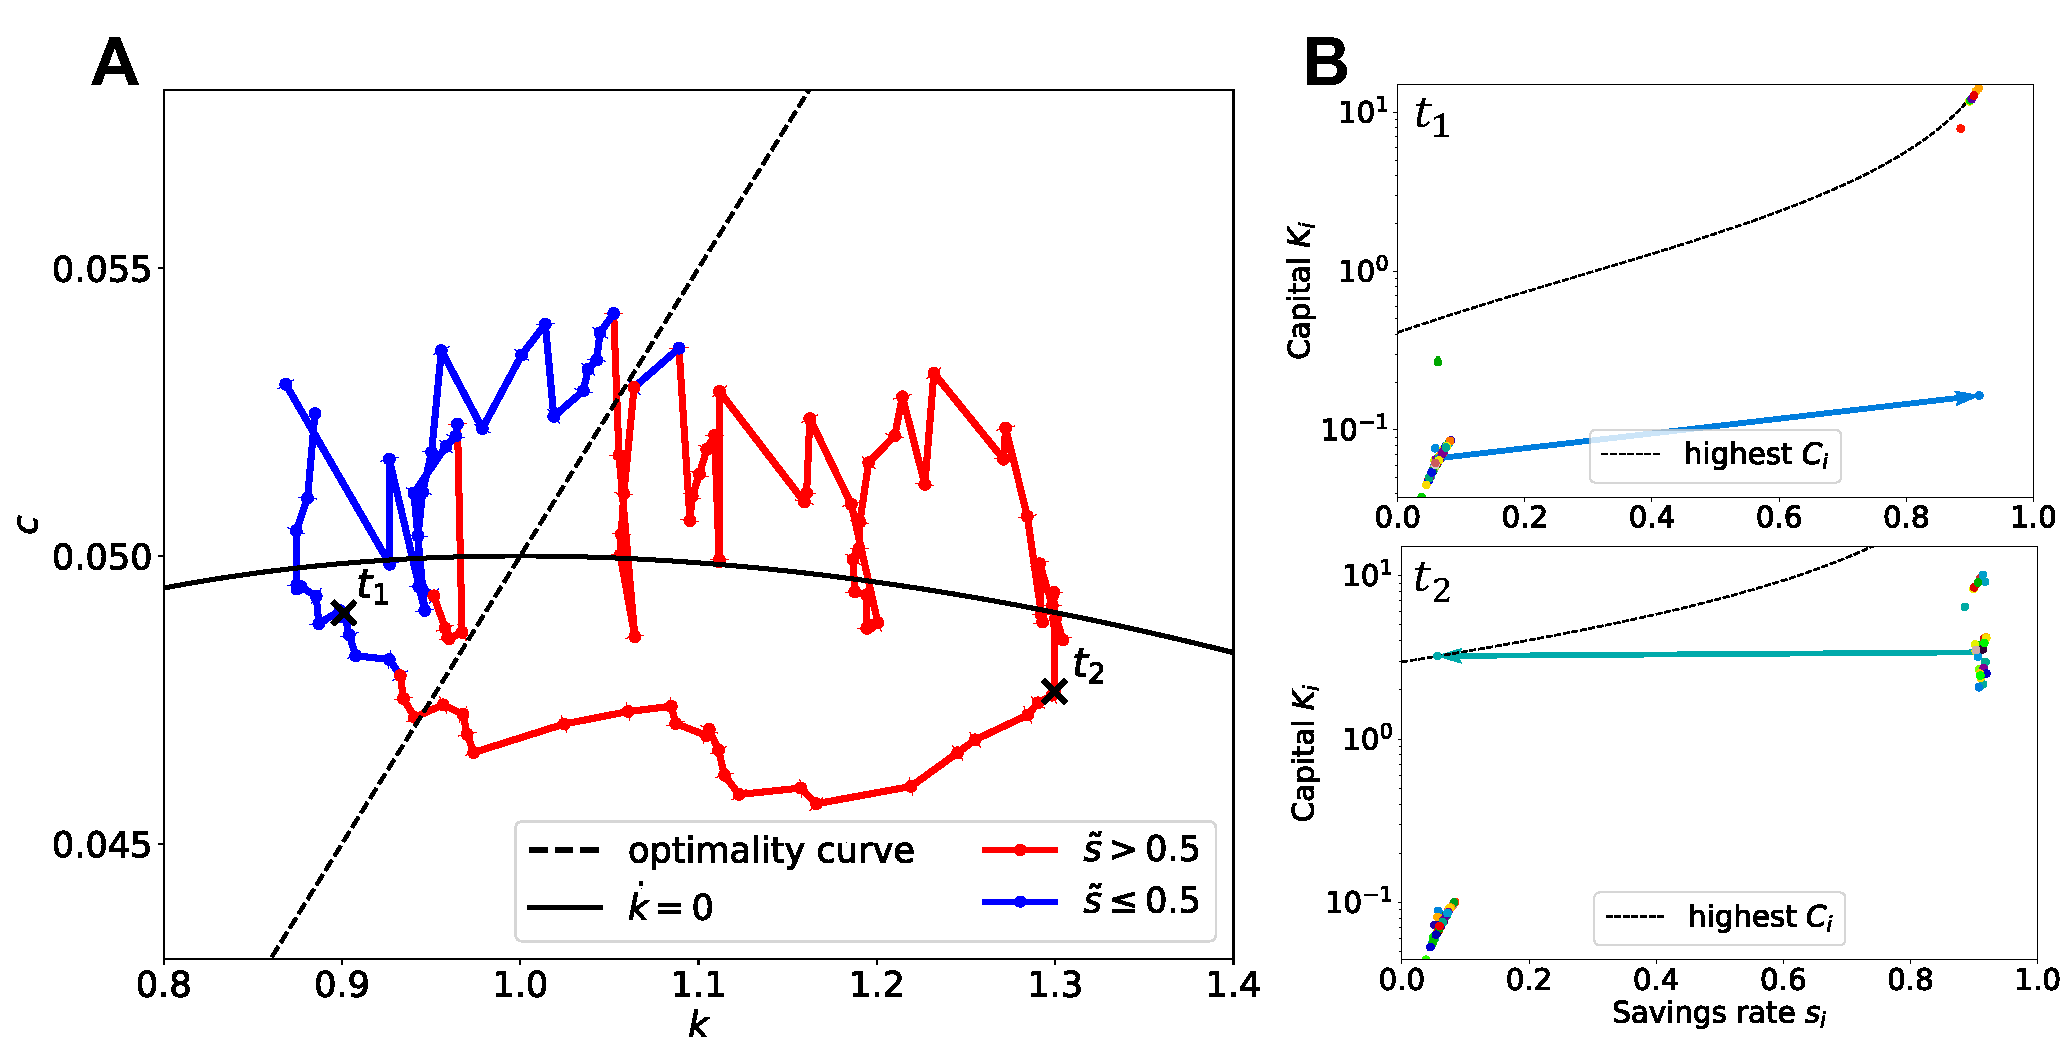
\includegraphics[width=0.98\textwidth]
       {figures/fig3.pdf}
       \caption{{ Endogenous dynamics in the oscillatory regime. } \textbf{A}: the average per-capita consumption $c$ against the average per-capita capital $k$. The aggregate saving rate $\tilde{s}$ is red when it is greater than $0.5$ and blue when it is less than $0.5$. The trajectory orbits around the optimal steady state $(k^\ast,c^\ast)$  of the standard RCK model, which is at the intersection of the dashed optimality curve (the solution to the standard RCK model discussed in sec.~\ref{sec:rck_stable}) and the solid black $\dot{k}=0$ line. Each dot corresponds to one household updating its savings rate; the direction of the orbit is counterclockwise.
\textbf{B}:~An illustration of the cause of the oscillatory dynamics.  The two panels show snapshots at two different times as indicated in figure A.  At time $t_1$ the aggregate savings rate is low, aggregate capital is low and the economy is in a depression; at time $t_2$ the opposite is true.  The capital and savings rates of individual households are shown as dots with different colors.  There are two clusters, corresponding to rich and poor households.  The household that is currently switching its savings rate is indicated by an arrow connecting its previous state to its current state.  The dashed black curve indicates the iso-consumption curve for the household $i$ with the highest consumption. }
\label{fig:dynamics}
\end{figure} 


In order to obtain a deeper understanding of the oscillatory regime, where $\tau > \tau_{c}$, fig.~\ref{fig:dynamics} illustrates both collective and individual dynamics.

Fig.\,\ref{fig:dynamics}A shows the average per capita consumption rate $c$ as a function of the average capital $k$. 
This illustrates how the aggregate consumption and capital orbit around the optimal steady state $(k^\ast,c^\ast)$  of the standard RCK model, generating a business cycle. 
The dashed line in fig.~\ref{fig:dynamics} represents the trajectory of the standard RCK model as discussed in sec.~\ref{sec:rck_stable}, the so called optimality curve, that is also depicted as the stable saddle point manifold in fig.~\ref{fig:rck_phase_space}.
In relation to the optimal savings rate $s^\ast \!=\!0.5$ of the RCK model, the effective aggregate savings rate $\tilde{s}$ of the modified model is typically greater than $s^\ast$ when the system is below the optimality curve and less than $ s^\ast$ when it is above the optimality curve. This means that when the heterogeneous households together have less capital than the representative household on the optimal trajectory, they increase their aggregate savings rate above the savings rate of the optimal scenario and vice versa, as if they were trying to collectively control their economy to steer it towards the optimal trajectory.
This is interesting as the optimality curve is obtained by assuming that a representative household optimizes its consumption for an infinite horizon, whereas in this modified model the individual household is oblivious of the mechanics of the economic system in which it operates and its behavior is myopic.

To understand the model mechanics at the individual level, fig.~\ref{fig:dynamics}B shows a snapshot of the capital vs.~the savings rate for all households at two different times, $t_1$ and $t_2$. 
At time $t_1$ the economy is just beginning to recover from a recession i.e. a period of low aggregate savings resulting in the depreciation of the capital stock and consequently lowered aggregate economic output. 
There are two clusters of households, corresponding to wealthy households with high capital $K_i$ and high savings rate $s_i$ and poor households with low capital $K_i$ and low savings rate $s_i$.
More households are poor, and because the return $r$ is inversely proportional to total capital according to $r \propto K^{-1 + \alpha}$, where here $\alpha = 0.5$, this means that returns to investment are high. 
As a consequence of this, wealthy households have a relatively higher consumption than poor households despite the fact that they save a large fraction of their income. This makes high savings rates comparatively more attractive than low savings rates. 
When the household shown in blue gets its chance to update its savings rate, it copies the higher savings rate of one of the rich households and moves in the $(K_i, s_i)$ plane as indicated by the arrow. Consequently, it begins accumulating capital by saving more.
Other households follow, and eventually the economy reaches the state shown in the lower panel at time $t_2$, where many houses have high savings rates and are rich.
The resulting excess capital drives the returns on savings down, which when combined with their high savings rates, depresses the consumption of these households.
As a result, when one of the rich households gets its turn to update, it copies a household with a low savings rate and goes on a spending spree.  

At this point its consumption rate becomes very high, and all of its neighbors copy it, creating a boom in consumption while decreasing the aggregate savings rate and consequently depreciating the capital stock of the economy.
A majority of households eventually become impoverished, returns on capital recover, high savings rates become more attractive again and the cycle repeats itself.
\newpage
\subsection{Critical Social Interaction Time}
\label{sec:savings_critical_tau}

What determines the critical social interaction time $\tau_\mathrm{c}$?
This question can best be answered by a closer analysis of eq. \eqref{eq:Citau} which describes the consumption of an individual household after time $\tau$ given that this household sets its savings rate $s_i$ individually relative to the constant aggregate savings rate $\tilde{s}$. 
\begin{wrapfigure}[27]{I}{.6 \textwidth}
  \centering
  \hspace{-1.5cm}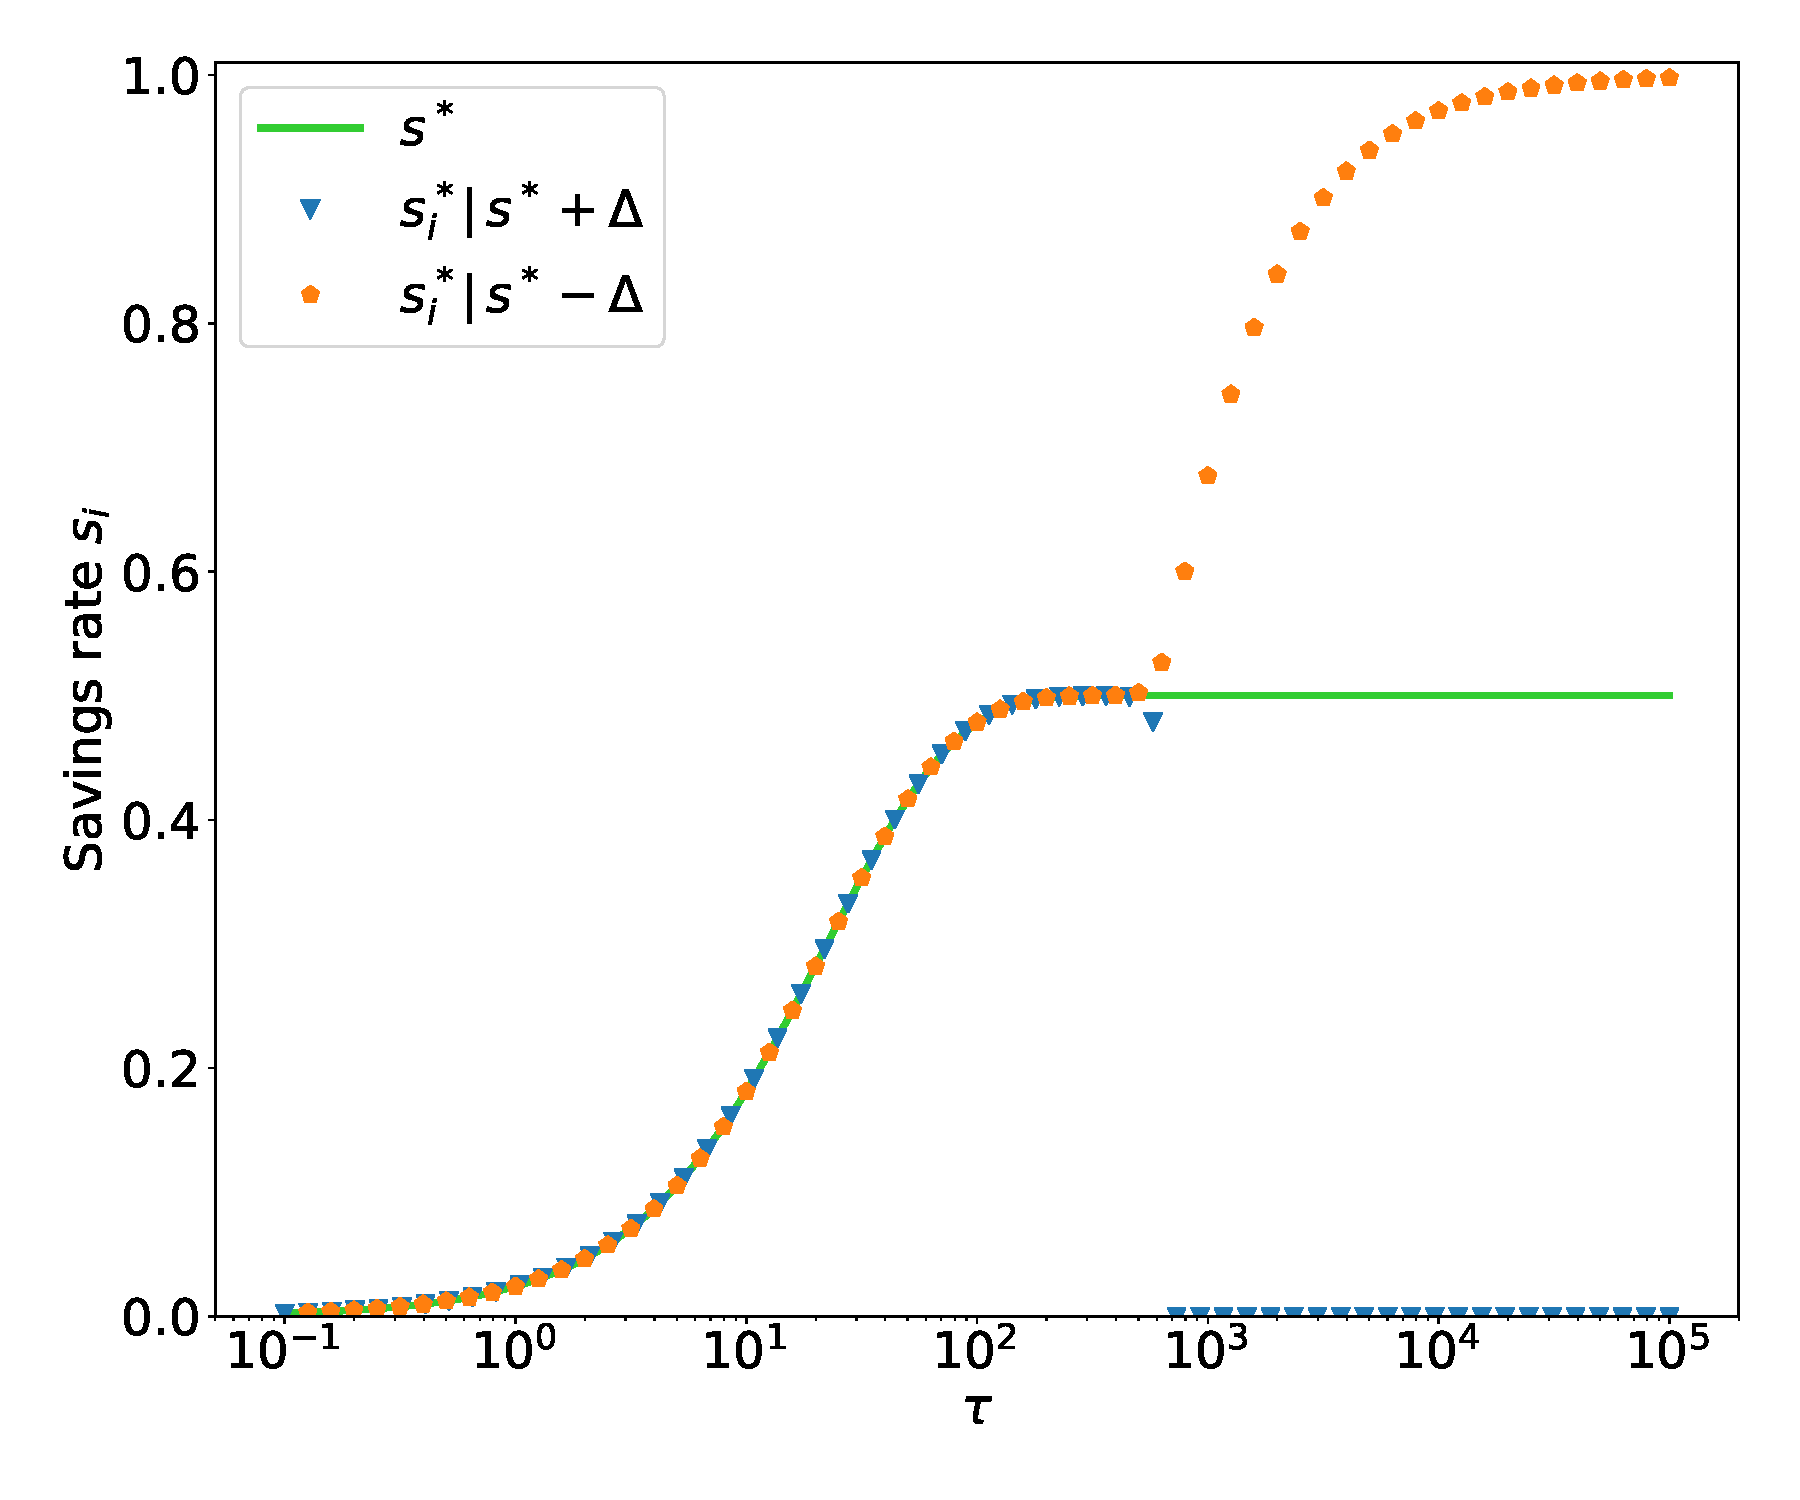
\includegraphics[width = .7 \textwidth]{figures/best_response.pdf}
  \caption{Best response dynamics. Optimal individual savings rate $s_i^\star$ (circles and triangles) given a very small perturbation of either $+\Delta$ (blue circles) or $-\Delta$ (orange triangles) of the aggregate savings rate $s$ away from its equilibrium value $s^\star$ (green line) as a function of the social interaction time $\tau$, for $\Delta = 10^{-7}$.}\hspace{.5cm}
  \label{fig:best_response}
\end{wrapfigure}

In section \ref{sec:rck_stable}, the analysis of this approximate equation showed that the imitate-the-best heuristic can result in behavior that is collectively ``optimal'' over a time horizon $\tau$ as it maximizes aggregate consumption. 
The reasoning behind this analysis also helps to understand the instability driving the transition: Eq.~\eqref{eq:Citau} also determines the incentives of a single household to set its individual savings rate equal to, close to, or far from the aggregate savings rate to maximize its individual consumption. 
Suppose that an external shock of size $\Delta$ perturbs the aggregate savings rate $\tilde{s}$ away from its collectively optimal value $s^\ast$, and suppose that household $i$ is allowed to optimize its savings rate $s_i$ while the others hold theirs constant. 
I call this optimal savings rate $s^*_i$ the \emph{best response} of the individual household. 
As displayed in fig. \ref{fig:best_response}, a numerical investigation shows that when $\tau \ll \tau_{c}$ i.e. in the \emph{stable regime}, the best response $s^*_i$ that maximizes the individual household's consumption after $\tau$ remains close to $\tilde{s}$. 
In contrast, when  $\tau \gg \tau_{c}$ e.g. in the \emph{oscillatory regime}, if $\Delta > 0$ then the individual household's best response $s^*_i$ is very small, with $s_i$ approaching $0$, and if $\Delta < 0$ the optimal savings rate is large, with $s_i$ approaching $1$. 


This happens because when $\Delta > 0$ the aggregate savings rate is high, so the returns on investment are low, which discourages saving and vice versa, when $\Delta < 0$ the aggregate savings rate is low, so returns on investment are high, which encourages saving. 
This destabilizes the unimodal solution around $s^\ast$. 
The transition occurs sharply at a parameter value near $\tau_{c}$, though the precise value depends on $\Delta$.
\newpage
\subsection{Dependence of the Critical Social Interaction Time on Network Size and Structure}  
\label{sec:savings_network_structure}

\begin{wrapfigure}[26]{I}{.6 \textwidth}
  \centering
  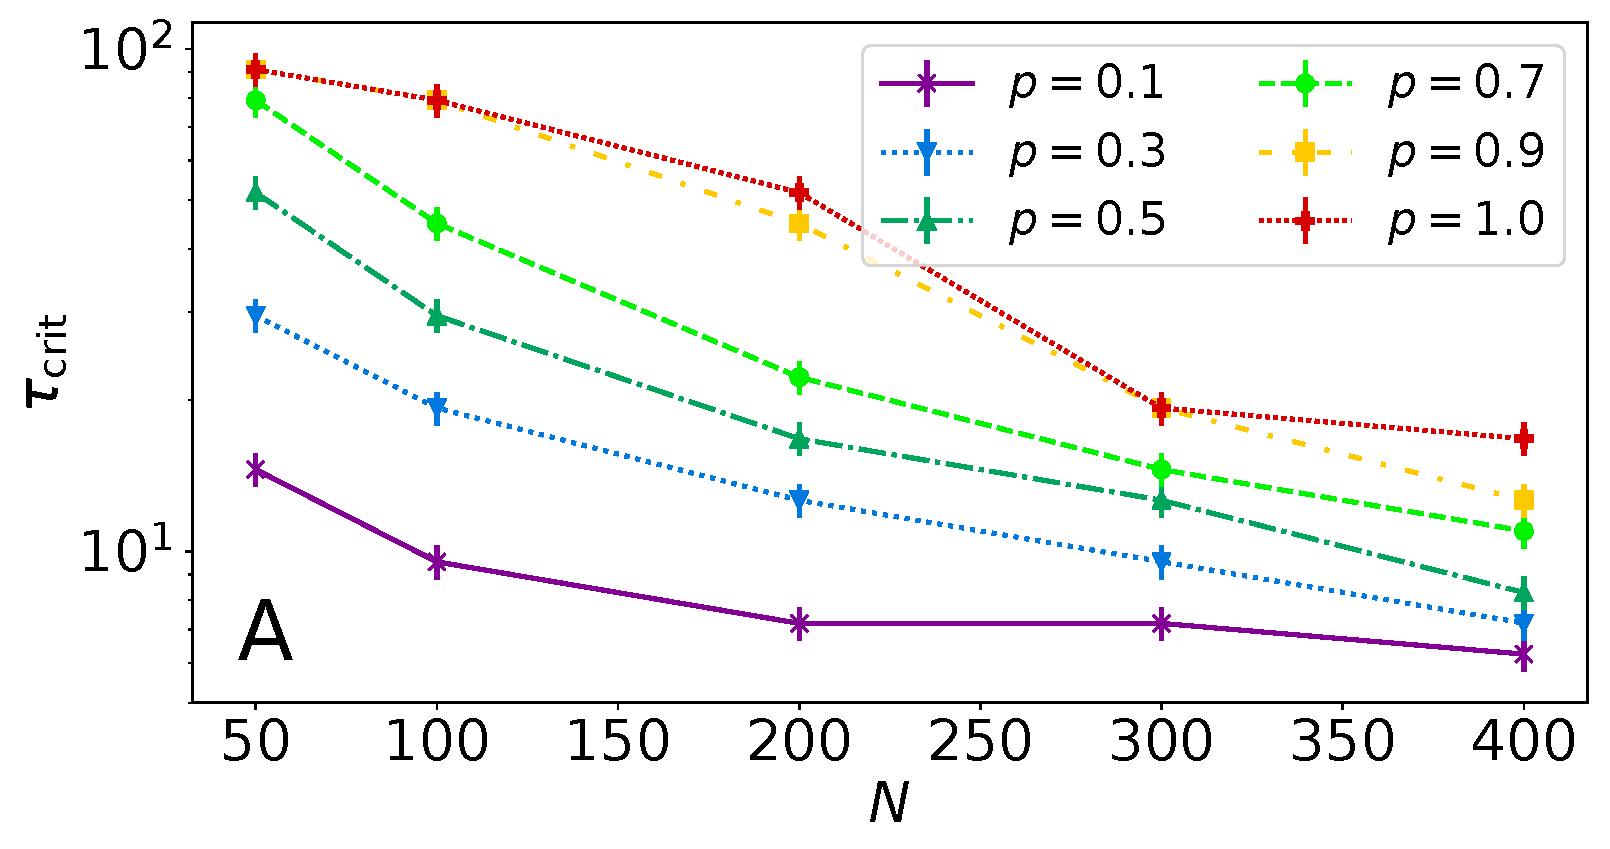
\includegraphics[width = .6 \textwidth]{figures/taucrit_N2.pdf}
  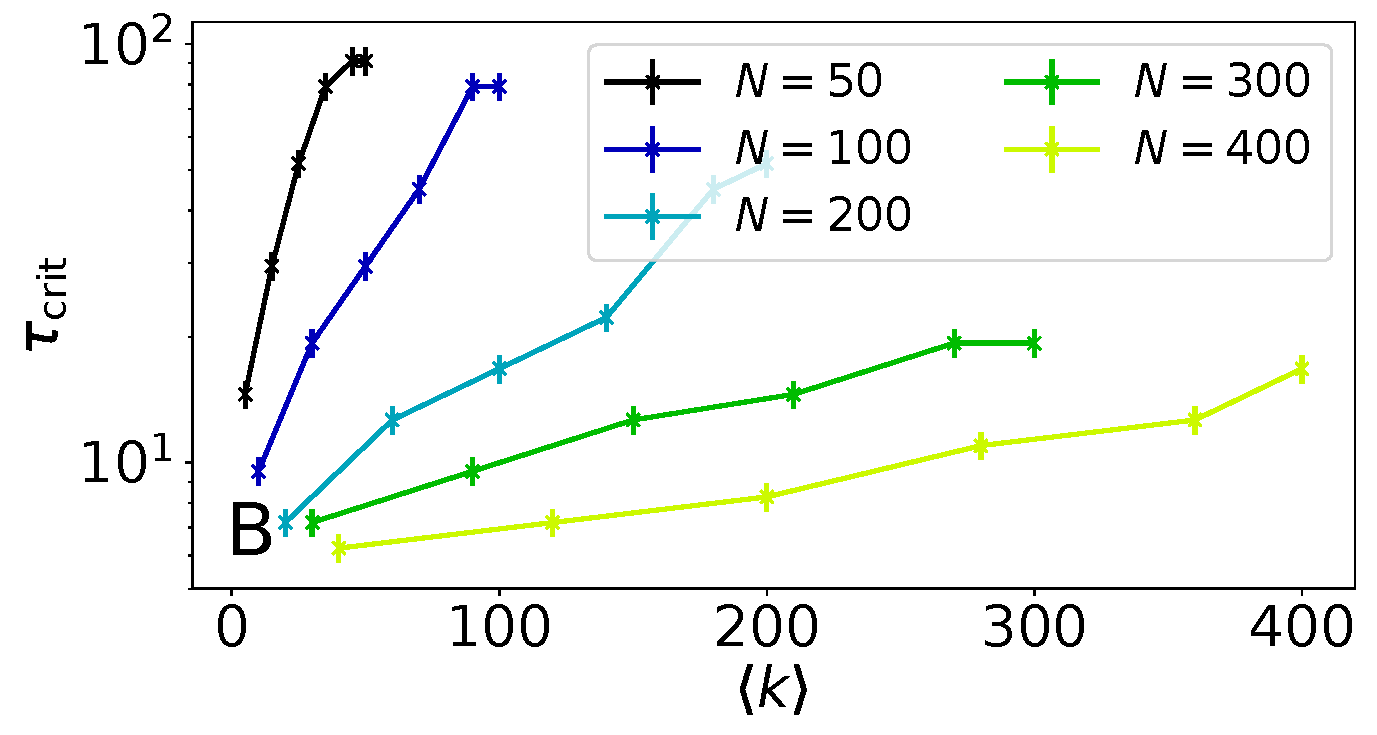
\includegraphics[width = .6 \textwidth]{figures/taucrit_N_k.pdf}
\caption{Critical interaction time $\tau_{crit}$ depending on A) network size $N$ for different link densities $p$ of the Erd\H{o}s-Renyi graph and B) mean degree $\left< k \right>$ for different network sizes $N$.}
  \label{fig:taucrit}
\end{wrapfigure}
The analysis of the incentives for the individual household to set its savings rate close to or far from the collectively optimal value $s^*$ in section \ref{sec:savings_critical_tau} gives a lower bound for the critical social interaction time. It shows that below a certain value for $\tau$ there is no benefit for the individual household in setting the savings rate far from the collectively optimal value. 
This analysis is agnostic of the network structure. However, in general the critical social interaction time also depends on the network size and structure. 
This can be illustrated using Erd\H{o}s Renyi networks where the average degree is $\langle k \rangle = (N-1)p \approx Np$, with $p$ being the probability that any two nodes are connected. Studying the model with this network topology shows that the critical social interaction time $\tau_{c}$ depends on both $N$ (fig. \ref{fig:taucrit}A) and $\langle k \rangle$ (fig. \ref{fig:taucrit}B). 

This can be understood by the following reasoning: Capital accumulation in the economic system has a specific time scale $t^* \propto 1/\alpha\delta$ (see section \ref{sec:full_dirty_economy}). This time scale determines the length of the time window during which an either high or low value of the savings rate leads to higher consumption and consequently spreads among the households. If in this time window eventually all households adopt the same savings rage, the bimodal distribution collapses to one of its branches. Then, households cannot make big changes to their savings rate anymore, since there are no households with a very different savings rate left that they could imitate.

What follows from this consideration is that the speed at which a signal propagates through the network via the models imitation process sets an upper limit to the critical social interaction time. This speed typically depends on the networks structural parameters such as mean degree of nodes $\langle k \rangle$ or average shortest path length through the network $\chi$.
Empirically, I finds the following proportional relationship between $\tau_c$, $\chi$, and $\langle k \rangle$:
\begin{equation}
\tau_c \sim e^{-\chi} / \langle k \rangle.
\label{scaling_relation}
\end{equation}  
Fig.\,\ref{taucrit} shows a fit of this relationship to various values for $\tau_{c}$.  Because $\chi$ increases with $N$, in the large $N$ limit the system is always in the oscillatory regime. Varying the network size and structure parameters also results in qualitative changes in the nature of the oscillation, affecting its frequency, amplitude and variability.

\begin{figure}[t]
     \centering
       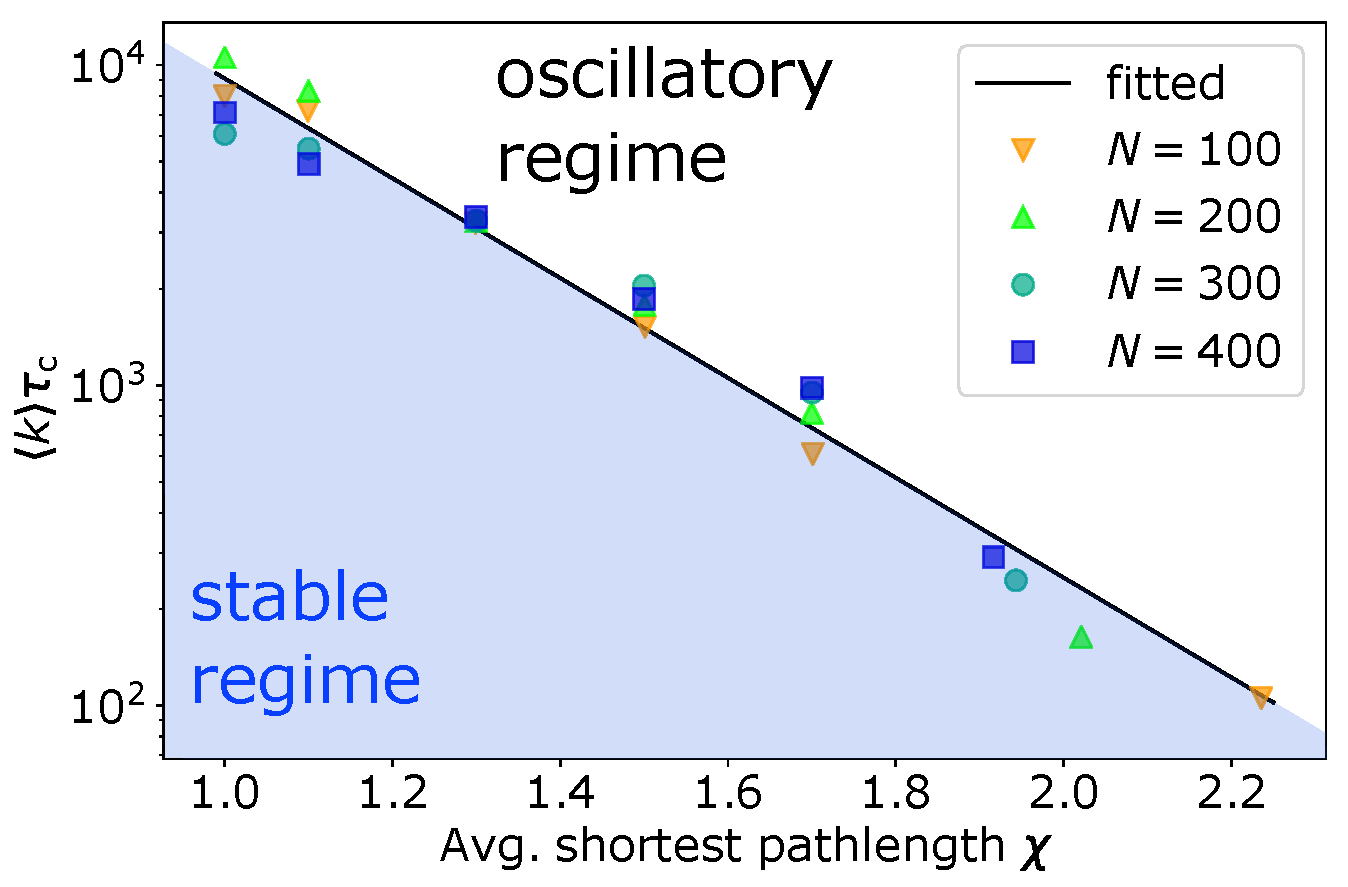
\includegraphics[width=0.8\textwidth]
       {figures/fig4.pdf}
	\caption{{The critical social interaction time depends on network properties.}
	The logarithm of the mean number of neighbors $\langle k \rangle$  times the critical interaction time $\tau_{c}$ is plotted vs. the average shortest path length $\chi$ for various values of $N$ and $p$, confirming eq.~\eqref{scaling_relation}. The stable regime ($\tau \! < \! \tau_{c}$) is shaded in blue. 
   \label{taucrit}}
\end{figure}

\section{Discussion and Conclusion}

The primary purpose of the analysis presented in this chapter was to investigate the possible implications of heterogeneous households individually setting their savings rates according to a simple behavioral heuristic. This analysis makes a somewhat surprising conceptual point by demonstrating how emergent inequality and endogenous dynamics can naturally emerge from a heterogeneous behavioral model. Despite its simplicity, the model accurately predicts that during recessions savings rates increase before output rises (see fig.~\ref{fig:micro_trajs}).
This has been observed for private savings in 19 OECD countries \citep{adema2015business}. 

Household savings rates are influenced by many things, and conspicuous consumption is only one of many factors. Standard macroeconomic models assume that agents are perfect utility maximizers, and attempt to provide realism by imposing frictions that restrict their behavior. Behavioral experiments, in contrast, indicate that real human beings are at best approximate utility maximizers.  Are the behaviorally observed deviations from utility maximization important for macroeconomics?  Can models that explicitly use behavioral rules capture features that standard models miss?

Absent shocks, standard macroeconomic models move toward an equilibrium and remain there.   Dynamics occur only because shocks knock the economy away from equilibrium. In this model, in contrast, the economy may display irregular endogenous oscillations that are reminiscent of business cycles.  
Although the model has the following two random inputs, they are small and very different in character from the shocks that drive the dynamics of standard models. The first random input determines the time at which individual households update their savings rates determined by a Poisson process. The timing of individual updates must be randomized to ensure that the order in which households update their savings rates varies\footnote{A fixed order leads to a static economy}. The second random input is the copying error for the savings rate.  This is small ($1\%$) and its exact value makes little difference to the behavior as long as it is nonzero. In contrast to standard shocks, which affect the economy as a whole, both of these inputs are at the level of individual households, and affect each household differently. For a large number of households the copying errors cancel out but the endogenous dynamics persist nonetheless. Thus while random inputs are necessary in this model, they do not directly drive booms and recessions as the shocks of standard models do. This is why the economic dynamics in this model can indeed be considered endogenous.

To illustrate the conceptual difference between this model and standard macroeconomic models it is useful to draw an analogy to a simple physical system. Consider the problem of pole balancing, in which a man attempts to move his hand to maintain a pole in a vertical position, as shown in fig.~\ref{pole_balancing}. The position of the man's hand corresponds to the collection of household savings decisions, and the pole/gravity system represents the economy or more precisely, the accumulation of capital in the economy. 
\begin{figure}
  \begin{minipage}[c]{0.5\textwidth}

	\caption[]{{ The problem of pole balancing is analogous to the problem of optimizing savings in an otherwise unstable economy.}  A man attempts to maintain a pole in a vertical position.  This is possible if the pole is long enough, but small errors in the control process drive endogenous oscillations in the angle of the pole.}
   \label{pole_balancing}
  \end{minipage}
  \begin{minipage}[c]{0.5\textwidth}
    \hspace{2 cm}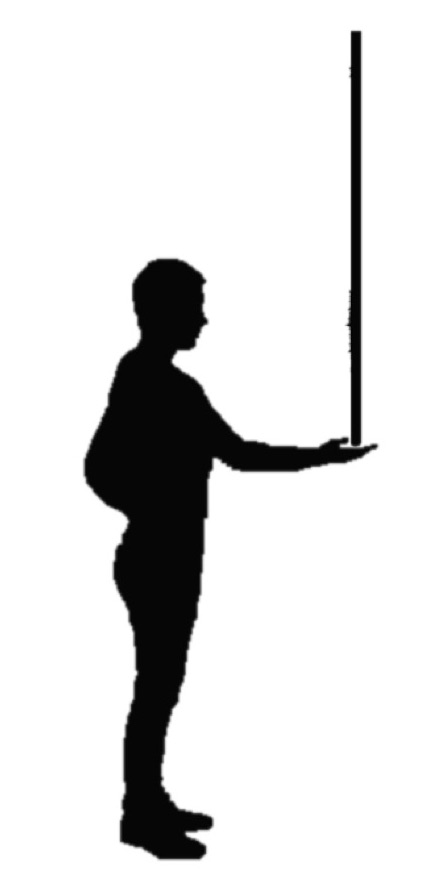
\includegraphics[width=0.3\textwidth]
       {figures/fig5.jpeg}
  \end{minipage}\hfill

\end{figure}
Short poles tip over more quickly than long poles, making it impossible to maintain a vertical position because the pole will tip over before the man can react.  If the pole is long enough, however, the man can move his hand to compensate, and maintain the pole in a roughly vertical position \citep{insperger2017stick}.  There is a sharp critical transition between stability and instability that occurs when the pole is about a meter in length\footnote{This is trivial to confirm empirically -- simply attempt to balance a pole of 60 cm. vs. 130 cm.}.
Nonetheless, even when the pole is rather long, it is not possible to maintain a perfectly vertical position, and the 
pole oscillates substantially.

An argument in the style of a standard macroeconomic model would posit that the man is a perfect pole balancer, and any deviations in the angle must be driven by external shocks, such as sharp gusts of wind, that suddenly cause the pole to deviate from vertical.  Under this view, after each shock the man moves his hand perfectly to make the pole vertical again as fast as possible, but before he can achieve this, another shock strikes it, making the pole oscillate around its vertical position.  For pole balancing it is clear that this explanation is wrong. Instead, theories that assume that oscillations are endogenously caused by imperfect control provide a better explanation for empirically observed behavior \citep{insperger2017stick}.
%Jobst reworded this to save space: provide a good explanation of the empirically observed behavior \cite{insperger2017stick}.  

The suggestion here is that the conceptual explanations for business cycles should be revisited as well.  This model adds weight to the idea that at least part of the variation in savings and investment that occurs during business cycles emerges endogenously due to the imperfect reasoning of households and firms.  The model also suggests that models incorporating agent heterogeneity might help illuminate the interaction between business cycles and inequality.  The fact that such rich behavior emerges from such a simple model supports a research agenda for macroeconomics based on empirically derived behavioral rules.

In the scope of this thesis, this chapter presents a surprisingly rich and interesting answer to a simple curious question. However, from the theoretical perspective, the analysis in this and the previous chapter were rather ad hoc. Although the results were interesting, analytical methods were only used to facilitate more efficient numerical analysis or as --- however well fitting --- still rudimentary approximation of model dynamics. Consequently the insights are limited to the specific cases that were studied. But it is apparent that both models have similarities with respect to the structure of interactions between individual agents. Namely, they both feature interactions between heterogeneous agents both on an individual basis that is structured by some form of network as well as through aggregated variables such as supply and demand.\footnote{This is also the case in many other socio-economic and social-ecological models that describe heterogeneous agents interacting with each other as well as aggregate market interaction, management of public goods of the state of a collectively managed resource.}. Also, in the broader view of describing bounded rational agents in \emph{whole} Earth models I want to better understand models like the ones presented in this and the previous chapter with analytical tools. This raises the question, whether a more general approach for an analytical description of the dynamical properties of these and other similarly structured models is possible. Consequently, in the subsequent chapter I develop an analytical approximation method for such models with networked heterogeneous agents that interact on an individual as well as on a mean field level.
